\documentclass[11pt]{beamer}

\usepackage[utf8]{inputenc}
\usepackage{amssymb}
\usepackage{hyperref}

\usetheme{Singapore}

\definecolor{DarkRed}{rgb}{0.50,0,0}
\definecolor{DarkGreen}{rgb}{0,0.50,0}
\definecolor{DarkBlue}{rgb}{0,0,0.50}
\definecolor{Black}{rgb}{0,0,0}

\newcommand{\ttdr}[1]{{\tt{\color{DarkRed} #1}}}
\newcommand{\emdr}[1]{{\em{\color{DarkRed} #1}}}
\newcommand{\ttdg}[1]{{\tt{\color{DarkGreen} #1}}}
\newcommand{\emdg}[1]{{\em{\color{DarkGreen} #1}}}
\newcommand{\ttdb}[1]{{\tt{\color{DarkBlue} #1}}}
\newcommand{\emdb}[1]{{\em{\color{DarkBlue} #1}}}

\setbeamertemplate{frametitle}{
  \begin{centering}
    {\Large \textbf{\textmd{\insertframetitle}}}
  \end{centering}
}

\setbeamertemplate{navigation symbols}{}

\setbeamertemplate{footline}{
  \begin{center}
    {\color{DarkBlue}{\large
        \insertframenumber}
      \hspace{280pt}
      
\includegraphics[height=20pt]{png/cycling.png}}
  \end{center}
}

\begin{document}



\begin{frame}
  \vspace{25pt}
  \begin{center}
    \LARGE{
      \vspace{10pt}
      {\color{DarkBlue}{
            Part One \\}}
      \vspace{10pt}
      Introduction
    }
  \end{center}
\end{frame}

\begin{frame}
  \frametitle{\begin{center}Notation\end{center}}
  \begin{itemize}
    \item<2-> using {\em math} language
    \begin{itemize}
      \item<3-> may be {\em difficult}
    \end{itemize}
    \item<4-> using {\em natural} language
    \begin{itemize}
      \item<5-> may be {\em ambiguous}
    \end{itemize}
    \item<6-> using {\em programming} language
    \begin{itemize}
      \item<7-> compiler understands it
      \item<8-> compiler rejects ambiguities that it cannot disambiguate 
    \end{itemize}
  \end{itemize}
\end{frame}



\begin{frame}[fragile]
  \frametitle{\begin{center}Category\end{center}}
  {\color{DarkGreen}
    \begin{verbatim}
  trait Category[BTC[_, _]]
    extends BtcComposition[BTC], BtcUnit[BTC]
    \end{verbatim}}
\end{frame}

\begin{frame}[fragile]
  \frametitle{\begin{center}Left Identity\end{center}}
  {\color{DarkGreen}
    \begin{verbatim}
  def leftIdentity[Z, Y]: BTC[Z, Y] => L[BTC[Z, Y]] = 
    z2y =>
      {
        i `o` z2y
      } `=` {
        z2y
      }
    \end{verbatim}}
\end{frame}

\begin{frame}[fragile]
  \frametitle{\begin{center}Right Identity\end{center}}
  {\color{DarkGreen}
    \begin{verbatim}
  def rightIdentity[Z, Y]: BTC[Z, Y] => L[BTC[Z, Y]] = 
    z2y =>
      {
        z2y `o` i
      } `=` {
        z2y
      }
    \end{verbatim}}
\end{frame}

\begin{frame}[fragile]
  \frametitle{\begin{center}Modeling time moments as real numbers\end{center}}
  \begin{itemize}
    \item<2-> traditionally we model time using real numbers and we take time limits,
              for example to define speed as a derivative, ds/dt, a limit of $\Delta$s/$\Delta$t,
              letting the sice of the interval $\Delta$t go to $0$, 
              which is possible in the mathematics \;\ldots\; but also in observed reality?
    \item<3-> below the Planck time unit we leave observable reality!
  \end{itemize}  
\end{frame}

\begin{frame}[fragile]
  \frametitle{\begin{center}Time\end{center}}
  {\color{DarkGreen}
    \begin{verbatim}
  trait Time[Moment: Arbitrary: Ordered]
    \end{verbatim}
  }
  \begin{itemize}
    \item<2-> this allows us to
      \begin{itemize}
        \item<3-> write statements involving arbitrary time moments
        \item<4-> state that one time moment is before another one
      \end{itemize}
  \end{itemize}
\end{frame}

\begin{frame}[fragile]
  \frametitle{\begin{center}orderedCategory\end{center}}
  {\color{DarkGreen}
    \begin{verbatim}
  given orderedCategory[
    Set[_]: Sets, // needed ???
    T: Arbitrary: Ordered
    ]
    : Category[[_, _] =>> Tuple2[T, T]] with

  type BTC = [_, _] =>> Tuple2[T, T]
    \end{verbatim}
  }
\end{frame}

\begin{frame}[fragile]
  \frametitle{\begin{center}orderedCategory\end{center}}
  {\color{DarkGreen}
    \begin{verbatim}
  extension [Z, Y, X](y2x: BTC[Y, X])
    def `o`(z2y: BTC[Z, Y]): BTC[Z, X] =
      (y2x, z2y) match
        case ((llt, lrt), (rlt, rrt)) =>
          require(
            llt `<=` lrt && lrt == rlt && rlt `<=` rrt
          )
          (llt, rrt)

  def i[Z]: BTC[Z, Z] =
    val at = summon[Arbitrary[T]].arbitrary
    (at, at)
    \end{verbatim}
  }
\end{frame}

\begin{frame}[fragile]
  \frametitle{\begin{center}Functor\end{center}}
  {\color{DarkGreen}
    \begin{verbatim}
  trait Functor[
    FBTC[_, _]: Category,
    TBTC[_, _]: Category,
    UTC[_]
  ]:
    def f[Z, Y]: 
      Function[
        FBTC[Z, Y],
        TBTC[UTC[Z], UTC[Y]]
      ]
    \end{verbatim}
  }
  \begin{itemize}
    \item<2-> {\color{DarkGreen}{\tt UTC}} is a {\em unary type constructor} parameter
   \end{itemize}
\end{frame}

\begin{frame}[fragile]
  \frametitle{\begin{center}Universe\end{center}}
  {\color{DarkGreen}
    \begin{verbatim}
  trait Universe[
    Set[_]: Sets,
    Morphism[_, _]: Category: ActingUponFunction,
    Moment: Time,
    State: [_] =>> VirtualTopology[
      Set, 
      State
    ]: [_] =>> Functor[
      // MomentMorphism instead???
      [_, _] =>> MomentMorphism, 
      Morphism,
      [_] =>> State
    ]
  ]
    \end{verbatim}
  }
\end{frame}

\begin{frame}[fragile]
  \frametitle{\begin{center}Universe\end{center}}
  \begin{itemize}
    \item<2-> this allows us to
      \begin{itemize}
        \item<3-> write statements using topological features of universe
          states
        \item<4-> write statements relating time moment morphisms, to
          universe state morphisms (think of dynamic universe states)
      \end{itemize}
  \end{itemize}
\end{frame}

\begin{frame}[fragile]
  \frametitle{\begin{center}PreThings\end{center}}
  {\color{DarkGreen}
    \begin{verbatim}
trait PreThings[
    Set[_],
    Morphism[_, _],
    Moment,
    State: [_] =>> Universe[
      Set,
      Morphism,
      Moment,
      State
    ],
    \end{verbatim}
  }  
\end{frame}

\begin{frame}[fragile]
  \frametitle{\begin{center}PreThings\end{center}}
  {\color{DarkGreen}
    \begin{verbatim}
    PreObject: [_] =>> Arbitrary[
      PreInteractionsSet
    ]: [_] =>> Functor[
      [_, _] =>> MomentMorphism,
      Function,
      [_] =>> PreThingsSet
    ]: [_] =>> Transformation[
      [_, _] =>> MomentTransition,
      Function,
      [_] =>> Set2[PreThingsSet],
      [_] =>> PreInteractionsSet
    ]: [_] =>> Function[PreThingsSet, State]
]:
    \end{verbatim}
  }  
\end{frame}

\begin{frame}
  \vspace{25pt}
  \begin{center}
    \LARGE{
      \vspace{10pt}
      {\color{DarkBlue}{
            Part Three \\}}
      \vspace{10pt}
      Laws of the non-existing reality
    }
  \end{center}
\end{frame}


\begin{frame}[fragile]
  \frametitle{\begin{center}An example: immobility\end{center}}
  \begin{itemize}
    \item<2-> immobility can be expressed without mentioning real numbers for
      time and space
    \item<3-> some history of geometry
      \begin{itemize}
        \item<4-> Euclides did not use numbers to measure with
        \item<5-> Pythagoras showed that rational numbers were not enough
      \end{itemize}
  \end{itemize}
\end{frame}

\begin{frame}[fragile]
  \frametitle{\begin{center}immobileAfter\end{center}}
  {\color{DarkGreen}
      \begin{verbatim}
  val immobileAfter
    : MomentMorphism => L[Function[PreThingsSet, State]] =
  mm =>
    {
      pts2s `o` mm2ptsf(mm)
    } `=` {
      mm2sm(mm) `a` pts2s
    }
      \end{verbatim}
}
\end{frame}

\begin{frame}[fragile]
  \frametitle{\begin{center}immobileAfter\end{center}}
  {\color{DarkGreen}
      \begin{verbatim}
  val immobileOnInterval
    : MomentMorphism 
        => PreThingsSet 
          => L[State] =
    case (bm, em) =>
      val mi: Interval[Moment] = 
        interval apply ((bm, em))
      \end{verbatim}}
\end{frame}

\begin{frame}[fragile]
  \frametitle{\begin{center}immobileAfter\end{center}}
  {\color{DarkGreen}
      \begin{verbatim}
      pts => // possible without pts ???
        all apply {
          for {
            m <- mi
          } yield {
            {
              (pts2s `o` mm2ptsf((bm, m)))(pts)
            } `=` {
              (mm2sm((bm, m)) `a` pts2s)(pts)
            }
          }
        }
      \end{verbatim}}
\end{frame}

\begin{frame}[fragile]
  \frametitle{\begin{center}Reality goes beyond Imagination\end{center}}
  \begin{itemize}
    \item<2-> the \ttdg{`a`} in the formula is not morphism composition
      \ttdg{`o`}
    \item<3-> the \ttdg{`a`} in the formula is an action of morphism
      \ttdg{mm2sm(mm)} on the place function \ttdg{pts2s}
    \item<4-> cfr a monoid acting upon a set
    \item<5-> cfr rotations acting upon a Rubic Cube
  \end{itemize}
\end{frame}

\begin{frame}[fragile]
  \frametitle{\begin{center}Type System\end{center}}
  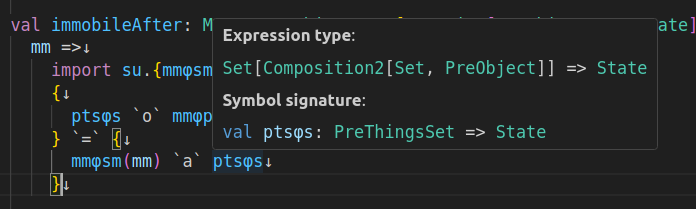
\includegraphics[height=100pt]{png/preThingSetToStateFunction.png}
  \vspace{40pt}
  \includegraphics[height=100pt]{png/stateToStateMorphism.png}
\end{frame}

\begin{frame}[fragile]
  \frametitle{\begin{center}More Information\end{center}}
  \ttdg{https://github.com/LucDuponcheelAtGitHub/timeHybrids}
\end{frame}

\begin{frame}[fragile]
  \frametitle{\begin{center}THANKS FOR ATTENDING\end{center}}
  \begin{center}
    
\includegraphics[height=190pt]{png/cycling.png}
  \end{center}
\end{frame}

\end{document}
